\documentclass[a4 paper]{article}
\usepackage[inner=2.0cm,outer=2.0cm,top=2.5cm,bottom=2.5cm]{geometry}
\usepackage{setspace}
\usepackage[ruled]{algorithm2e}
\usepackage[rgb]{xcolor}
\usepackage{verbatim}
\usepackage{subcaption}
\usepackage{amsgen,amsmath,amstext,amsbsy,amsopn,tikz,amssymb}
\usepackage{fancyhdr}
\usepackage[colorlinks=true, urlcolor=blue,  linkcolor=blue, citecolor=blue]{hyperref}
\usepackage[colorinlistoftodos]{todonotes}
\usepackage{rotating}
\usepackage{booktabs}


\newcommand{\ra}[1]{\renewcommand{\arraystretch}{#1}}

\newtheorem{thm}{Theorem}[section]
\newtheorem{prop}[thm]{Proposition}
\newtheorem{lem}[thm]{Lemma}
\newtheorem{cor}[thm]{Corollary}
\newtheorem{defn}[thm]{Definition}
\newtheorem{rem}[thm]{Remark}
\numberwithin{equation}{section}

\newcommand{\homework}[6]{
	\pagestyle{myheadings}
	\thispagestyle{plain}
	\newpage
	\setcounter{page}{1}
	\noindent
	\begin{center}
		\framebox{
			\vbox{\vspace{2mm}
				\hbox to 6.28in { {\bf MATH 118:~Statistics and Probability \hfill {\small (#2)}} }
				\vspace{6mm}
				\hbox to 6.28in { {\Large \hfill #1  \hfill} }
				\vspace{6mm}
				\hbox to 6.28in { {\it Instructor: {\rm #3} \hfill Name: {\rm #5} \hfill Student Id: {\rm #6}} \hfill}
				\hbox to 6.28in { {\it Assistant: #4  \hfill #6}}
				\vspace{2mm}}
		}
	\end{center}
	\markboth{#5 -- #1}{#5 -- #1}
	\vspace*{4mm}
}

\newcommand{\problem}[2]{~\\\fbox{\textbf{Problem #1}}\hfill (#2 points)\newline\newline}
\newcommand{\subproblem}[1]{~\newline\textbf{(#1)}}
\newcommand{\D}{\mathcal{D}}
\newcommand{\Hy}{\mathcal{H}}
\newcommand{\VS}{\textrm{VS}}
\newcommand{\solution}{~\newline\textbf{\textit{(Solution)}} }

\newcommand{\bbF}{\mathbb{F}}
\newcommand{\bbX}{\mathbb{X}}
\newcommand{\bI}{\mathbf{I}}
\newcommand{\bX}{\mathbf{X}}
\newcommand{\bY}{\mathbf{Y}}
\newcommand{\bepsilon}{\boldsymbol{\epsilon}}
\newcommand{\balpha}{\boldsymbol{\alpha}}
\newcommand{\bbeta}{\boldsymbol{\beta}}
\newcommand{\0}{\mathbf{0}}

\usepackage{listings}
\usepackage{color}

\definecolor{dkgreen}{rgb}{0,0.6,0}
\definecolor{gray}{rgb}{0.5,0.5,0.5}
\definecolor{mauve}{rgb}{0.58,0,0.82}

\lstset{frame=tb,
  language=Python,
  aboveskip=3mm,
  belowskip=3mm,
  showstringspaces=false,
  columns=flexible,
  basicstyle={\small\ttfamily},
  numbers=none,
  numberstyle=\tiny\color{gray},
  keywordstyle=\color{blue},
  commentstyle=\color{dkgreen},
  stringstyle=\color{mauve},
  breaklines=true,
  breakatwhitespace=true,
  tabsize=3
}

\begin{document}
	\homework{Homework \#2}{Due: 07/06/21}{Dr. Zafeirakis Zafeirakopoulos}{Gizem S\"ung\"u}{}{}
	
	\subproblem{d} Draw a barplot for the actual cases (Table \ref{tab2} in column 2) and the predicted cases (Table \ref{tab2} column 3) with respect to \# of defecrs. You should put the figure.\\

    \centering
    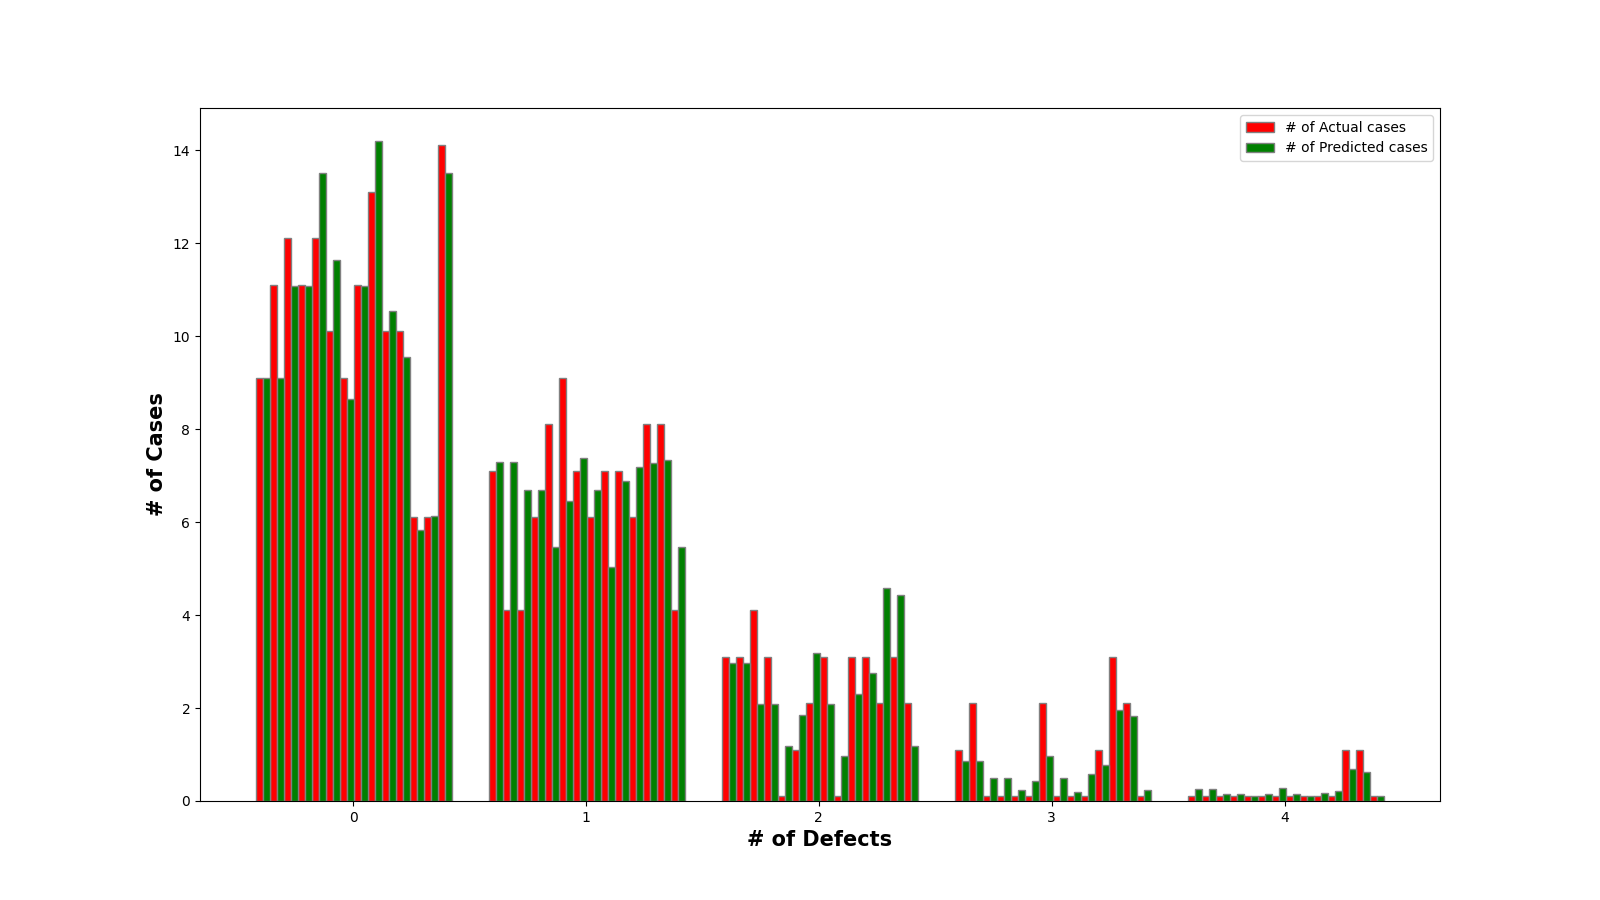
\includegraphics[scale = 0.4]{hw2_figure.png}
	
	\subproblem{e} According to the barplot in (d), does the poisson distribution fit the data well? Compare the values of the actual cases and the values of the poisson predicted cases, and write your opinions about performance of the distribution.\\
	
	\begin{itemize}
	    \item 
	    There is a margin of error close to 0.1 between the total observed case and total the predicted case. In most companies, the estimated number and the actual number are very close to each other. There is some difference between predicted and observed datas in some manufacturers' datas, but not much. As a result of these, we can say that by looking at the table; The poisson distribution does fit the data well. By looking at the closeness of the predicted values to the observed values, we can say that the poisson distribution performs well.
	\end{itemize}
	
	\subproblem{f} According to your estimations above, write your opinions considering your barplot and Table \ref{tab2}. Which company do you prefer to buy a car? Why?\\
	\begin{itemize}
	    \item 
	    I prefer 9th company to buy a car. The reason is that 9th company has excess number of 0 states and less problems in cases 2, 3 and 4 than others. The observed cases being less than or equal to the predicted cases, except in the case 1.  
	    
	\end{itemize}
	
	\subproblem{g} Paste your code that you implemented for the subproblems above. Do not forget to write comments on your code.\\
	Example:\\
	\begin{itemize}
		\item The common code block for all subproblems\\
		Paste here. Your code should read the file and compute other things which the following subproblems need.\\
		\begin{lstlisting}
		# Python file

		  import csv
        from math import factorial
        import numpy as np
        import matplotlib.pyplot as plt

        with open("manufacturing_defects.txt", 'r') as myFile:
            csv_reader = csv.reader(myFile, delimiter='\t')
            data = []

            for row in csv_reader:
                if len(row) != 0:  # The last row is empty in given file, to skip this and likely rows.
                    data.append(row)
                
		\end{lstlisting}
		\newpage
        
		\item
		The code block for (a)\\
		Paste here. Your code should compute the values in Table 1 column 2.
		\begin{lstlisting}
  def p_a():

    result = []
    temp = []
    j = 2  # first manufacturer.
    while j < 16:
        zero_count = 0
        one_count = 0
        two_count = 0
        three_count = 0
        four_count = 0
        for i in data:
            if i[j] == "0":
                zero_count += 1
            elif i[j] == "1":
                one_count += 1
            elif i[j] == "2":
                two_count += 1
            elif i[j] == "3":
                three_count += 1
            elif i[j] == "4":
                four_count += 1
        result.append([zero_count, one_count, two_count, three_count, four_count])
        j += 1

    return result

#  prints the table
def print_p_a():  # [[0, 1, 2, 3, 4], [0, 1, 2, 3, 4], .....]
    table = p_a()
    j = 0

    print("\n# of Defects", end=" ")
    print("   # of cases in all company between the years \n")
    while j < 5:
        print('{:<15}'.format(j), end=" ")  # After the 0, 1, 2, 3 and 4 cases, it puts 5 empty character.
        for i in table:
            print('{:<3}'.format(i[j]), end=" ")  #  {:>5} To align rows. It prints organized.
        j += 1
        print("")
    print("\nTable 1: Actual cases")
		\end{lstlisting}
		
		\item The code block for (b)\\
		Paste here. Your code should compute $\lambda$.
		
		\begin{lstlisting}
def my_lambda():  #  0 * numbers of 0  + 1 * numbers of 1 + 2 * numbers of 2 ... / 20
    table = p_a()
    lambdas = []
    for i in table:
        sum = 0
        k = 0
        for j in i:
            sum += (k*j)
            k += 1
        lambdas.append(sum/20)
    return lambdas

def poisson(lam, k): # (e**-lam) * ((lam*k)/k!)
    return (np.exp(1)**(-lam))*((lam**k)/factorial(k))
		\end{lstlisting}
		
		\item The code block for (c)\\
		Paste here. Your code should compute the values in Table 2 column 3.
		
		\begin{lstlisting}
def p_c():
    table = p_a()
    lambdas = my_lambda()
    result = []
    temp = []
    counter = 0
    for i in table:
        j = 0
        while j < 5:
            temp.append((poisson(lambdas[counter], j)*20))  #  prediction number -> ex. 0.45 * 20(year) -> 9 times
            j += 1
        result.append(temp)
        temp = []
        counter += 1
    
    return result


actual_cases = p_a()
predicted_cases = p_c()  # [[# of 0, # of 1, # of 2, # of 3, # of 4], [# of 0, # of 1, # of 2, # of 3, # of 4]

# this func prints table 2 completely
def print_act_predic(actual_cases, predicted_cases):  # [[0, 1, 2, 3, 4], [0, 1, 2, 3, 4], .....]
    j = 0
    print("\n# of Defects", end=" ")
    print("   # of cases in all company between the years", end=" ")
    print("                  Predicted # of cases in all company between the years \n")
    while j < 5:
        print('{:<15}'.format(j), end=" ")  # after the 0, 1, 2, 3, 4 cases, it puts 5 empty character
        for i in actual_cases:
            print('{:<3}'.format(i[j]), end=" ")  #  {:>5} # To align through below.
        print("     ", end=" ")
        for i in predicted_cases:
            print('{:<6.2f}'.format(round(i[j], 2)), end=" ")  #
        
        j += 1
        print("")
    print("\nTable 2: Actual vs. Predicted Cases")
		\end{lstlisting}
		
		\item The code block for (d)\\
		Paste here. Your code should draw the barplot.
		\begin{lstlisting}
def barplot(actual_cases, predicted_cases):
    #  In this part we add 0.1 to all datas since all datas will be shown in the graph. 
    # Otherwise, 0 values does not appear.
    
    i = 0
    j = 0
    while i < len(actual_cases):
        while j < len(actual_cases[0]):
            actual_cases[i][j] += 0.1
            j += 1
        i += 1
        j = 0

    i = 0
    j = 0
    while i < len(predicted_cases):
        while j < len(predicted_cases[0]):
            predicted_cases[i][j] += 0.1
            j += 1
        i += 1
        j = 0

    barWidth = 0.03
    fig = plt.subplots(figsize=(16, 9))

    # Set position of bar on X axis
    br1 = [0, 1, 2, 3, 4]
    br2 = [x + barWidth for x in br1]
    br3 = [x + barWidth for x in br2]
    br4 = [x + barWidth for x in br3]
    br5 = [x + barWidth for x in br4]
    br6 = [x + barWidth for x in br5]
    br7 = [x + barWidth for x in br6]
    br8 = [x + barWidth for x in br7]
    br9 = [x + barWidth for x in br8]
    br10 = [x + barWidth for x in br9]
    br11 = [x + barWidth for x in br10]
    br12 = [x + barWidth for x in br11]
    br13 = [x + barWidth for x in br12]
    br14 = [x + barWidth for x in br13]
    br15 = [x + barWidth for x in br14]
    br16 = [x + barWidth for x in br15]
    br17 = [x + barWidth for x in br16]
    br18 = [x + barWidth for x in br17]
    br19 = [x + barWidth for x in br18]
    br20 = [x + barWidth for x in br19]
    br21 = [x + barWidth for x in br20]
    br22 = [x + barWidth for x in br21]
    br23 = [x + barWidth for x in br22]
    br24 = [x + barWidth for x in br23]
    br25 = [x + barWidth for x in br24]
    br26 = [x + barWidth for x in br25]
    br27 = [x + barWidth for x in br26]
    br28 = [x + barWidth for x in br27]

# Make the plot

    plt.bar(br1, actual_cases[0], color='r', width=barWidth, edgecolor='grey', label='# of Actual cases')
    plt.bar(br3, actual_cases[1], color='r', width=barWidth, edgecolor='grey')
    plt.bar(br5, actual_cases[2], color='r', width=barWidth, edgecolor='grey')
    plt.bar(br7, actual_cases[3], color='r', width=barWidth, edgecolor='grey')
    plt.bar(br9, actual_cases[4], color='r', width=barWidth, edgecolor='grey')
    plt.bar(br11, actual_cases[5], color='r', width=barWidth, edgecolor='grey')
    plt.bar(br13, actual_cases[6], color='r', width=barWidth, edgecolor='grey')
    plt.bar(br15, actual_cases[7], color='r', width=barWidth, edgecolor='grey')
    plt.bar(br17, actual_cases[8], color='r', width=barWidth, edgecolor='grey')
    plt.bar(br19, actual_cases[9], color='r', width=barWidth, edgecolor='grey')
    plt.bar(br21, actual_cases[10], color='r', width=barWidth, edgecolor='grey')
    plt.bar(br23, actual_cases[11], color='r', width=barWidth, edgecolor='grey')
    plt.bar(br25, actual_cases[12], color='r', width=barWidth, edgecolor='grey')
    plt.bar(br27, actual_cases[13], color='r', width=barWidth, edgecolor='grey')
    plt.bar(br2, predicted_cases[0], color='g', width=barWidth, edgecolor='grey', label='# of Predicted cases')
    plt.bar(br4, predicted_cases[1], color='g', width=barWidth, edgecolor='grey')
    plt.bar(br6, predicted_cases[2], color='g', width=barWidth, edgecolor='grey')
    plt.bar(br8, predicted_cases[3], color='g', width=barWidth, edgecolor='grey')
    plt.bar(br10, predicted_cases[4], color='g', width=barWidth, edgecolor='grey')
    plt.bar(br12, predicted_cases[5], color='g', width=barWidth, edgecolor='grey')
    plt.bar(br14, predicted_cases[6], color='g', width=barWidth, edgecolor='grey')
    plt.bar(br16, predicted_cases[7], color='g', width=barWidth, edgecolor='grey')
    plt.bar(br18, predicted_cases[8], color='g', width=barWidth, edgecolor='grey')
    plt.bar(br20, predicted_cases[9], color='g', width=barWidth, edgecolor='grey')
    plt.bar(br22, predicted_cases[10], color='g', width=barWidth, edgecolor='grey')
    plt.bar(br24, predicted_cases[11], color='g', width=barWidth, edgecolor='grey')
    plt.bar(br26, predicted_cases[12], color='g', width=barWidth, edgecolor='grey')
    plt.bar(br28, predicted_cases[13], color='g', width=barWidth, edgecolor='grey')

# Adding Xticks
    plt.xlabel('# of Defects', fontweight='bold', fontsize=15)
    plt.ylabel('# of Cases', fontweight='bold', fontsize=15)
    plt.xticks([r + barWidth + 0.37 for r in range(5)], ['0', '1', '2', '3', '4'])

    plt.legend()
    plt.show()		
		\end{lstlisting}
		
	\end{itemize}
	
	
	
	
\end{document} 


